\section{Intervention Locations}
\label{sec:accessing_records}

\begin{figure*}[t]
	\centering
	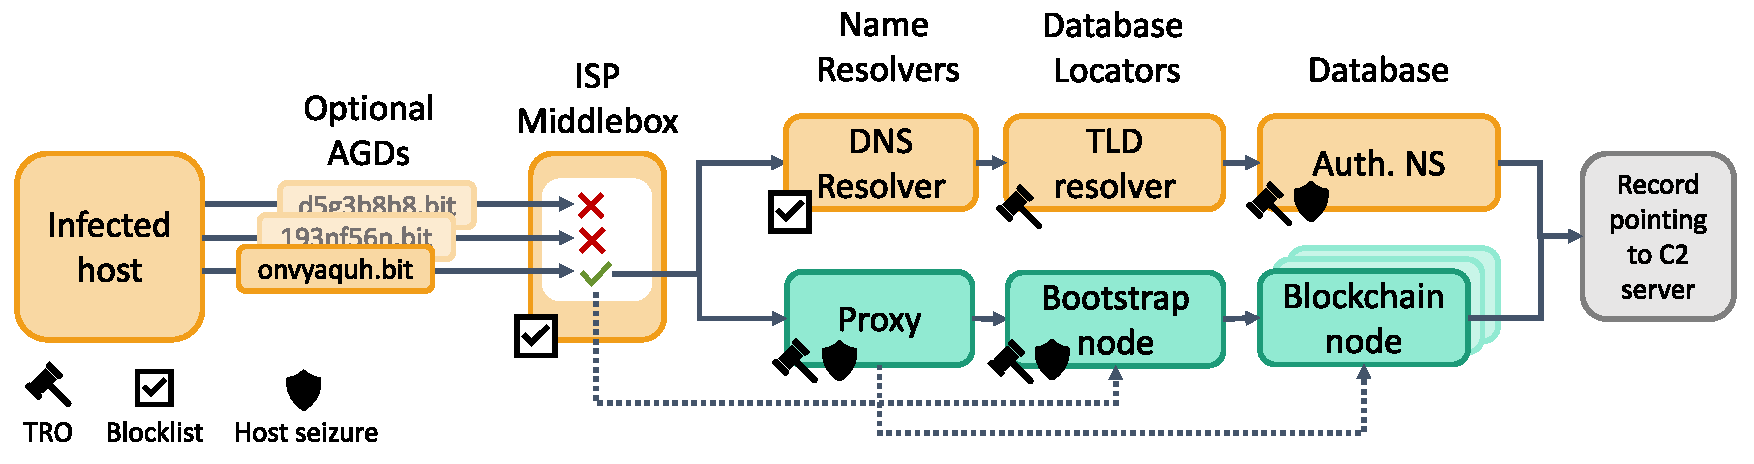
\includegraphics[width=\textwidth]{figs/intervention_locations.pdf}
	\caption{Potential locations of interventions for 
	blocking access to DNS-based and blockchain-based C2 
	server names.}
	\label{fig:malware_contacting_cnc}
\end{figure*}

Accessing any naming system, whether blockchain-based or DNS-based, requires a 
number of steps, each of which presents an opportunity for defenders to stage 
an intervention. Figure~\ref{fig:malware_contacting_cnc} compares the 
steps an infected host takes to resolve a DNS C2 domain 
(shown in orange) to 
the steps required to resolve a blockchain 
name (shown in green). While these steps involve different participants, 
parallels exist between the blockchain and DNS ecosystems. 
Figure~\ref{fig:malware_contacting_cnc} also details the interventions that 
can be staged by defenders at each step of the process. We now describe each 
step and its potential interventions in detail. For certain interventions at 
certain steps, we also present a case study of an attempt to stage the 
intervention in the wild, its results, and the lessons it provides for 
defenders. 

\subsection{Reaching the resolver}

Regardless of whether a request is destined for DNS or a 
blockchain naming 
system, it must first reach the machine that acts as a 
resolver: either the DNS 
resolver or the proxy in 
Figure~\ref{fig:malware_contacting_cnc}. Defenders may 
be able to intervene before this point by placing middleboxes 
with filter lists 
in the network. Some networks already have such defenses: for 
example, some ISP 
networks redirect all DNS requests to the ISP's own resolver, 
which can 
implement a filter list. This defense is probably not 
currently intended to 
block blockchain names, but it has that effect nevertheless 
in some cases. For example, some malware uses 
ordinary DNS rather than DNS-over-HTTPS to request blockchain 
domains, under 
the assumption that the proxy the query is intended for will 
redirect it to the 
blockchain naming system in the correct format. When ISPs 
perform DNS 
redirection to their own resolvers, these queries get 
redirected to the DNS 
root, which cannot resolve the alt-TLDs used by blockchain 
naming systems and return ``NXDOMAIN.'' We 
present our study of this phenomenon in 
Section~\ref{sec:b-root}. We observe 
that filter lists are only a partial defense against malware, 
because malware may utilize DGAs to evade them: as soon as a 
C2 name is added to the blocklist, the malware operators may 
register and begin using a new one. 

\subsection{Interventions at the name resolver}

When resolving DNS domains, the entity that first attempts to 
respond to the request is a DNS resolver. When using 
blockchain naming systems, this entity is a proxy instead, 
shown in Figure~\ref{fig:malware_contacting_cnc} under ``Name 
Resolvers.'' The proxy
may expect queries in 
the form of DNS-over-HTTPS, unencrypted DNS, or in an 
arbitrary format. Instead of querying the DNS root zone, the 
TLD resolver, and eventually the authoritative nameserver to 
resolve a name, the proxy must connect to the blockchain and 
retrieve the record from one of the participants.
Defenders may intervene at a traditional DNS resolver by requesting that the 
resolver implement a filter list, or the resolver operators may elect to 
implement one voluntarily. However, proxies that resolve blockchain names may 
be resistant to such voluntary efforts, because the blockchain ecosystem is 
often organized around principles of independence and self-governance, and 
resistance exists to the idea of censoring any content.

Proxies are currently the most common method for resolving 
blockchain names. Table~\ref{tab:proxies_and_tlds} shows a 
selection of the proxies and tools that resolve names from 
each of the systems we study. The list of proxies is not 
exhaustive, but represents 
a subset of the best-known proxies in use at the time of 
writing. While most large 
browsers, such as Safari, Chrome, and Firefox, do not support 
any blockchain naming systems natively, some naming systems 
provide browser extensions that redirect blockchain name 
queries to proxies using DoH. A few browsers do resolve 
blockchain names without requiring extensions, such as Brave, 
which partners with a proxy called 
Infura~\cite{brave_uses_infura}. Some naming systems have 
partnerships with existing DNS resolvers. For example, 
NextDNS's DNS resolvers can act as proxies to resolve 
Handshake names. Finally, some naming systems, such as 
Handshake, also provide stub resolver implementations that 
run locally on a user's computer. These stub resolvers also 
work by routing blockchain name queries to proxies.

Almost all of these proxies are centralized, in that they 
are controlled by a single authority. This is good 
news for defenders: similarly to traditional registrars, they 
are vulnerable to legal takedowns. They can be served with 
TROs or warrants and compelled to stop giving access to 
abused domains, as long as they operate within a jurisdiction 
amenable to such efforts. A centralized proxy could also be 
neutralized by serving a takedown order to its 
hosting provider, although this approach would produce 
varying amounts of the collateral damage depending on how 
many licit users utilize the proxy. 
While these interventions are not 
foolproof, they are subject to the same advantages and 
disadvantages as interventions on traditional registrars. 
Thus, centralized proxies return the distributed naming 
ecosystem to a state similar to the DNS ecosystem, from a 
defender's point of view. 

\subsubsection{Case Study \#1 --- OpenNIC ceasing support of \texttt{.bit}}

OpenNIC is one of the few decentralized proxy services for 
blockchain names. It resolves names from several alternative 
naming systems, including Namecoin and 
Emercoin~\cite{opennic}. OpenNIC's 
resolvers are run by a small community of 
volunteers~\cite{opennic_servers}. In June 2019, this 
community voted of their own volition to remove support for 
Namecoin's \texttt{.bit} alt-TLD, because providers were 
beginning to block OpenNIC resolvers that were used by 
malware to resolve Namecoin 
names~\cite{opennic_namecoin_vote}.

OpenNIC's decision to cease supporting Namecoin was not the 
result of a direct intervention by defenders, but it still 
yields an important lesson. Even a decentralized proxy 
service may be composed of few enough individuals that it is 
possible to cajole or compel them to stop resolving names 
used by malware. Furthermore, OpenNIC's community held this 
vote in response to pressure from Spamhaus, Malwarebytes, and 
other providers, who began blocklisting OpenNIC resolver 
domains: even if a proxy's operators cannot be contacted 
directly, it is still possible to pressure them to cease 
resolving names used by malware.

\subsubsection{Case Study \#2 --- BDNS takedown}

In April 2021, various defenders attempted to take down a proxy known as 
``Blockchain-DNS.info'' or BDNS. BDNS reported on their website soon after the 
takedown attempt 
that seven of their domain names had been ``un-delegated'' 
and one of their API servers was shut down without 
warning~\cite{blockchain-dns-info-wayback}. For example, one 
endpoint, \texttt{bdns.io}, was 
apparently sinkholed by ShadowServer~\cite{shadowserver}. 
\texttt{bdns.io}'s NS 
records now point to variants of the name 
\texttt{sinkhole.shadowserver.org}.\footnote{sinkhole-0[0-4].shadowserver.org
	and sinkhole-[a-b].shadowserver.org.} We confirmed that these 
NS records were 
changed to ShadowServer's domains on March 26, 2021, using 
the pDNS 
database~\cite{domaintools_pdns}. BDNS 
received a message from Spamhaus shortly after noticing the 
takedown, stating that several of 
BDNS's endpoint domains had been added to Spamhaus's 
blocklist. BDNS 
claimed that their browser extensions continued to resolve 
blockchain names using other endpoints, and directed users to 
a list of endpoints that were still 
working~\cite{github_bdns_wayback}. BDNS also stated that 
they had moved some infrastructure to a friendlier hosting 
provider, PRQ, which states on its website that ``If 
[content] is legal in Sweden, we will host it, and will keep 
it up regardless of any pressure to take it 
down''~\cite{prq}. However, as of August 2022, all of the endpoints 
listed in BDNS's 
Github repository~\cite{github_bdns_wayback} are either 
failing to resolve or resolving but failing to 
load content, and the proxy appears to be nonfunctional.

This takedown effort provides several lessons for defenders. 
First, defenders must take care when choosing a takedown 
strategy for a proxy. In this case, defenders tried two 
tactics: 
adding the proxy's endpoints to a widely used blocklist and 
taking down some domains and a hosting server entirely. 
The former tactic appeared to work well in locations where 
ISPs use Spamhaus's blocklist: BDNS stated that their 
proxy ``may be still unreachable in those parts of the 
world.'' However, the domain takedown appeared to be 
only partially effective, since BDNS could still resolve 
blockchain names for a time using unaffected endpoints. We 
conclude that 
care must be taken to enumerate all of a proxy's endpoints 
and shut them down simultaneously.  



\subsection{Skipping the proxy: the rise of light clients}

While proxies greatly simplify the process of 
connecting to a blockchain, they are not strictly necessary, 
which is bad news for defenders. We initially assumed that no infected host 
would be able to 
skip the proxy and participate directly 
in the blockchain, because acting as a blockchain node 
requires too many resources. However, this assumption turned 
out to be incorrect, because of the rise of \emph{light 
clients}. When blockchains were first envisioned, most 
assumed that every participant in the network would be a 
``full'' implementation of a node: it would contain 
enough state to reconstruct the entire history of the chain, 
all the way back to the first transaction. Additionally, each 
node would contribute to the 
blockchain by verifying every transaction it heard about. As 
blockchains grow over time, they become too 
resource-intensive to run on anything other than a dedicated, 
powerful machine. Two resources serve as 
the constraints: first, CPU power, which is obviously 
necessary to perform mining but now is even a bottleneck for 
transaction verification, because so many transactions happen 
per second. Second, disk space and speed: for example, a full 
Ethereum node cannot be run on a machine with a hard disk 
drive anymore, because nothing slower than a solid state 
drive can keep up with the reads and writes 
required~\cite{geth_faq}. These 
resource constraints make it 
very unlikely that malware could run ``full'' blockchain 
nodes on infected hosts. However, these constraints have also
given rise to the concept of a ``light client,'' a blockchain 
node with limited functionality that can fetch transactions 
from the chain but does not contribute by verifying 
transactions, mining, or broadcasting. Light clients are 
designed to run on laptops and mobile devices. As such, they 
use few enough resources to reasonably be included in 
malware. 


\subsection{Interventions at the Database Locator}

Light clients enable malware to act as a first-class member 
of a blockchain, and discover other members of the chain 
using the chain's peer-to-peer discovery protocol without 
using a centralized proxy. In this case, 
defenders are left 
with a harder location to stage an intervention: the 
blockchain's bootstrap nodes, which is the blockchain 
equivalent of a service that locates the database of naming 
records. 
We show this path in 
Figure~\ref{fig:malware_contacting_cnc} with the dotted line 
between the middlebox and the bootstrap nodes. 

In traditional DNS, the resolver must locate the database 
that contains a record by first querying the hierarchy of DNS 
servers: first the root and then the TLD resolver. The TLD 
resolver's role is to tell the DNS resolver which machine 
stores the database that ultimately contains a name's 
records. In a blockchain system, this role is filled by the 
bootstrap nodes. The purpose of the bootstrap 
nodes is to provide a gateway to the blockchain for new 
participants: new blockchain nodes find their initial list of 
potential peers by connecting to the bootstrap nodes. 
Blockchains use various methods to publish bootstrap 
node addresses for their users. For 
example, Ethereum uses a list of bootstrap nodes 
that are hard-coded into 
client implementations~\cite{geth_bootstrap}. Bitcoin 
stores lists of bootstrap nodes in DNS TXT records maintained 
by volunteers, as 
well as hard-coded 
lists~\cite{bitcoin_bootstrap}.

When defenders perform interventions by putting legal 
pressure on registrars, the intervention takes effect at the 
TLD resolver, which implements the changes to the zone file 
that affect the malware's domains. These changes can include 
``sinkholing'' the domain by causing it resolve to an IP 
controlled by defenders or ``freezing'' it so that 
its records cannot be modified. This intervention does not 
translate well to blockchain naming systems for several 
reasons. 

First, while bootstrap nodes are responsible for finding the 
entire naming database, they do not allow defenders to 
specify which blockchain systems a client may access and 
which it may not. This means that seizing a specific naming 
record, or even the entire naming system, is not possible at 
the bootstrap nodes. Consequently, disabling or seizing 
bootstrap nodes prevents all new clients from accessing any 
functionality provided by the blockchain, including the 
blockchain's cryptocurrencies and any services it offers 
unrelated to naming. This approach therefore carries the 
potential for a lot of collateral damage. Second, bootstrap 
nodes may be widely distributed across the globe, leading to 
jurisdictional challenges in bringing legal pressure to bear 
on their operators. Bootstrap nodes may also be difficult to 
find, since they may not be run by hosting providers but 
rather by anonymous individual volunteers. Third, bootstrap 
nodes may be numerous enough that finding and seizing them 
all may be prohibitively difficult. Finally, while the 
default bootstrap node lists are published for each 
blockchain, users may choose to substitute their own. A 
malware author could design a payload that contains an 
extensive list of machines that participate in a blockchain 
naming system, which would complicate a defender's efforts to 
take down all the potential participants. Because 
interventions at the bootstrap nodes are more challenging 
than interventions at the proxy, we show the intervention 
icons in gray in Figure~\ref{fig:malware_contacting_cnc}.

However, defenders could fall back to using blocklists at 
network middleboxes to deny access to bootstrap nodes. For 
example, IDSes, enterprise firewalls, or ISP routers can drop 
traffic intended for bootstrap nodes. This approach is very 
similar to blocking any other 
malicious IP addresses, and is subject to the usual 
challenges. Defenders must keep blocklists up-to-date as 
malware authors update the IPs they connect to. To the 
advantage of defenders, any time malware authors 
are forced to update the IP addresses that bootstrap nodes 
may be found at, they run afoul of the ``sunk cost'' problem 
where infected machines that cannot be updated become
useless. A similar argument applies if malware chooses to 
access bootstrap nodes using hard-coded DNS domain names 
instead of hard-coded IP addresses. Additionally, 
traditional interventions against domain names apply in that 
situation as well. Thus, while intervening at bootstrap nodes 
poses more of a challenge than intervening at centralized 
proxies, defenders still have viable options to choose from.

\subsection{Interventions at the Database}

In traditional DNS, defenders can sinkhole the domain of an 
authoritative nameserver or seize the server itself to 
prevent malware accessing a C2 domain record. This 
intervention is impractical for blockchain names, 
because instead of a single machine acting as the 
authoritative nameserver, every blockchain node has a copy of 
the database. Seizing the database would require either taking down 
every machine in the blockchain, or executing a successful ``51\%'' attack by 
taking control of more than half of the computing power in the blockchain. 
Blockchains are generally highly robust against attacks like these, which makes 
them unlikely to be the most practical intervention for defenders to attempt. 
However, small naming-specific
blockchains with few participants may be more vulnerable. 

\subsubsection{Case Study \#3 --- Namecoin's Vulnerability to 51\% Attacks}

Like all of the naming-specific blockchains that we study, the Namecoin 
blockchain has many fewer participants than blockchains like Ethereum. This 
makes Namecoin more vulnerable than larger blockchains to a ``51\%'' attack. A 
51\% attack can be executed when an attacker controls more 
than half of the 
computational power of the blockchain, allowing them to rewrite historical 
transactions or add invalid ones. Gaining control of more than half of a 
blockchain's computational power is much easier on blockchains with few 
participants. 

Namecoin has already experienced problems in this area. As of 2014, one mining 
pool known as ``DiscusFish'' or ``F2Pool'' consistently controlled more than 
60\% of the computational power of Namecoin, and on 
occasion controlled up to 75\%~\cite{ali2016blockstack}. While we 
did not find any reports that F2Pool had attacked Namecoin, they had the 
capability to do so. This vulnerability suggests two 
potential interventions. 
First, because Namecoin apparently has few licit 
users~\cite{casino_unearthing_2021}, 
interventions that render the entire naming system inoperable are more feasible 
than they would be on more popular general-purpose blockchains. Therefore, 
defenders could attempt to take over the entire blockchain and sinkhole 
all abused names by seizing control of F2Pool. Second, 
defenders could potentially 
apply legal pressure to the operators of F2Pool to coerce them to sinkhole 
certain specific names. This intervention would rely on 
defenders' ability to find 
F2Pool's operators and apply legal pressure in the jurisdiction the operators 
reside in. We predict that such an intervention would be challenging, but the 
fact that it appears possible at all contradicts the received wisdom that 
blockchains cannot be taken over directly. 

\subsection{Interventions after the name record is acquired}
\label{sec:interventions_at_name}

If an infected host successfully retrieves its C2 record, 
that record might take several forms. The three that we 
observed in existing blockchain naming systems that might be 
useful to malware were IP addresses, traditional DNS domains, 
and addresses for distributed storage systems like IPFS and 
SkyNet. Some naming 
systems also allow users to store arbitrary text as 
records, which would let malware operators store nonstandard 
record types like links to social media posts. 

Each of these record types are subject to all of the 
traditional interventions that have already 
been described, except one: DS addresses. Distributed storage 
systems provide a form of ``bulletproof'' hosting, under the limitation
that all hosted content must be static files and not dynamic 
websites. Any C2 server implemented entirely on such a 
system must be a simple file with no 
dynamic content. Infected hosts that wish to contact a distributed storage 
system must pass through the same steps shown in 
Figure~\ref{fig:malware_contacting_cnc} for accessing a blockchain, which means 
they are subject to the same interventions. For example, a strain of malware 
called ``IPStorm'' has already been discovered using IPFS for its C2 server in 
the wild. IPStorm connects to IPFS using bootstrap nodes~\cite{ipstorm_anomali, 
ipstorm_zdnet}, which may be seized or blocked.

Another advantage for defenders is that some distributed storage systems, 
such as IPFS, do not have redundancy: only a single machine hosts each piece of 
a file. This raises the possibility of discovering the particular machine 
responsible for hosting a C2 server and seizing it. 

A final possibility for intervening with the name record may be to seize 
names stored in ``hosted'' or ``custodial'' wallets. Some 
businesses, such 
as cryptocurrency exchanges, provide custodial wallets for 
users who wish to let 
the company handle their blockchain-based assets. This service is designed to 
make blockchain interaction easier for customers, but as a consequence, the 
business knows the custodial wallet's private key. If a name is stored in a 
custodial wallet, the business that runs the wallet 
could seize it~\cite{pegoraro_blockchain_2021}. However, a 
successful intervention must be difficult for malware operators to 
evade, and we note that malware operators with good operational practices can 
simply choose not to use custodial wallets. 

\subsection{Intervening with name modification or purchase}

Generally speaking, DNS domains are cheaper, easier to modify, and 
easier to replace than IP addresses, because each IP address 
represents a compromised machine while new domains can be 
purchased inexpensively. Blockchain-based domains on 
general-purpose chains, such as Bitcoin and Ethereum, 
change this norm. While resolving a name is free, malware 
operators must pay \emph{transaction fees} 
(known as \emph{gas fees} on Ethereum)
to register or modify names. These transaction fees 
can be quite expensive. For example, we found that 
registering a new name on the Unstoppable Domains service 
cost nearly \$80 in gas fees during a period of high fees. 
In contrast, the cost of the name itself was \$10. While 
licit users may wait for fees to be low at times of low 
network congestion, malware operators may not have that 
choice if they wish to avoid downtime in their campaign. High 
transaction costs poses challenges for defenders as well. For 
example, to combat DNS-based DGAs, defenders have the option 
of registering every domain the DGA will ever generate. This 
intervention would be much less practical if each 
registration was nearly an order of magnitude more expensive.

Naming-specific blockchains, such as Namecoin, Emercoin, and Handshake, 
present a different set of tradeoffs for defenders and malware 
operators. These 
blockchains are created with the sole intention of hosting a naming system. 
With fewer users and correspondingly less demand, these systems' names are 
usually much less expensive than names in Ethereum-based systems. This enables 
malware authors to use fast flux or DGA-based strategies, and also may enable 
defenders to pre-register domains generated by DGAs. 






%\subsection{Naming record formats}
%
%
%
%
%\randall{where do I put this? Additionally, because all 
%blockchain 
%	records 
%	are public, anyone can fetch those records including 
%	defenders. You could theoretically scrape a blockchain 
%looking for records 
%	that match a known 
%	malicious format or with malicious traits of some sort 
%(owned by the same 
%	wallet?) and try to seize 
%	whatever those records point to.} 
%
%
%
%I don't know if IPFS/SkyNet have light nodes that could be 
%part of a malware payload, but there does seem to be a trend 
%in that direction as chains get heavier.